\section*{Теоретические сведения}

Диффузия в системе из двух компонентов a и b подчиняется
закону Фика:
\begin{align}
    j_a = -D \frac{\partial n_a}{\partial x}; j_b = -D\frac{\partial n_b}{\partial x}
\end{align}
где $D$ - коэффициент взаимной диффузии компонентовt.\\\indent
В работе исследуется взаимная диффузия гелия и воздуха. 
Давление и температура предполагаются постоянными:
\begin{align}
    P = (n_{\text{He}} + n_{\text{в}})kT &= const \Rightarrow \\ 
    \Rightarrow \Delta n_{\text{в}} &= -\Delta n_{\text{He}}
\end{align}
\indent В работе концентрация гелия мала, к тому же атомы гелия легче молекул,
составляющих воздух. Поэтому перемешивание газов в работе можно приближенно
описывать как диффузию примеси легких частиц гелия на стационарном фоне воздуха. 
Тогда коэффициет диффузии равен:
\begin{align}
    D = \frac{1}{3}\lambda\overline{\upsilon}
\end{align}
где $\overline{\upsilon} = \sqrt{\frac{8 R T}{\pi\mu}}\text{ - средняя тепловая скорость частиц примеси;$\lambda$ - длига свободного пробега}$\\ 
\indent
Таким образом, теория предполагает обратную пропорциональность 
коэффициента взаимной диффузии двух газов и давления.\\

\section*{Экспериментальная установка}
\indent
\subsection*{Теоретические справки}
Для исследования взаимной диффузии газов и
измерения коэффициента взаимной диффузии D используется два сосуда
объёмами $V_1$ и $V_2$ ($V_1 \approx V_2$), соединенные трубкой длины L и сечения S.\\ 
\begin{wrapfigure}{r}
    \centering
    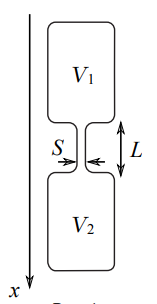
\includegraphics[height=5cm]{setup1.png}
    \caption{Сосуд}
\end{wrapfigure}
\indent
В трубке установится стационарный поток частиц, одинаковый в каждом 
сечении трубки, иначе частицы бы накапливались там, и процесс не был бы 
стационарным. Исходя из этих соображений можно записать:
\begin{align}
    j = -D\frac{\partial n}{\partial x} &= const \Rightarrow\\ 
    \Rightarrow n(x) &= \frac{\Delta n}{L}x\\ 
    j &= -D\frac{\Delta n}{L}
\end{align}
где $\Delta n$ - разность концентраций гелия на концах трубки.\\\indent
Также будем считать процесс квазистатическим, предполагая медленность его
протекания. Т.е время процесса должно оказаться намного больше времени 
диффузии отдельной частицы вдоль трубки длиной $L$ и сечением $S$. 
$\tau_{\text{диф}} \sim \frac{L^2}{2D} \ll \tau$
\begin{align}
    \frac{dN_1}{dt} &= jS\text{  ;  }\frac{dN_2}{dt} = -jS \Rightarrow\\ 
    \Rightarrow \frac{d(\Delta n)}{dt} &= -\frac{\Delta n}{\tau} \\ 
    \tau &= \frac{1}{D}\frac{VL}{2S}
\end{align}
Из уравнений выше получаем:
\begin{equation}
    \Delta n = \Delta n_0e^{-\frac{t}{\tau}}
\end{equation}
а также условие квазистатичности: $\tau_{\text{диф}} \ll \tau \Rightarrow SL \ll V$
\subsection*{Методика измерений}
\indent
\begin{wrapfigure}{i}
    \centering
    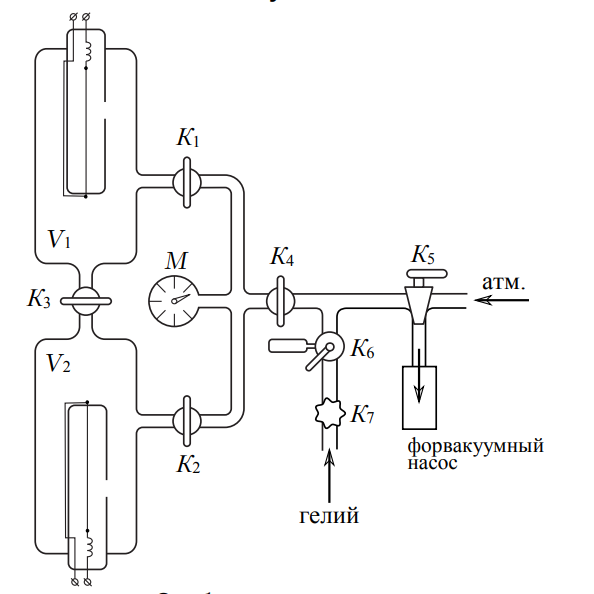
\includegraphics[width=7cm,height=7cm]{mainsetup.png}
    \caption{Экспериментальная установка}
\end{wrapfigure}


Для измерения разности концентраций в установке применяются датчики теплопроводности. 
Теплопроводность смеси зависит от ее состава и при малой разности $\Delta n$
можно ожидать, что разность теплопроводностей будет прямо пропорциональна $\Delta n$:
$\Delta k = k(n_2) - k(n_1) \approx const \cdot \Delta n$
Для измерения сопротивлений используется мостовая схема.
Мост балансируется при заполнении сосудов одной и той же
смесью. При заполнении сосудов смесями различного состава возникает
«разбаланc» моста. При незначительном различии в составах смесей показания вольтметра
будут изменяться по такому же закону, как и разность концентраций: 
$U = U_0e^{-\frac{t}{\tau}}$
Сама экспериментальная установк показана слева. 

\newpage

\begin{figure}[!h]
    \centering
    \begin{subfigure}{0.45\textwidth}
        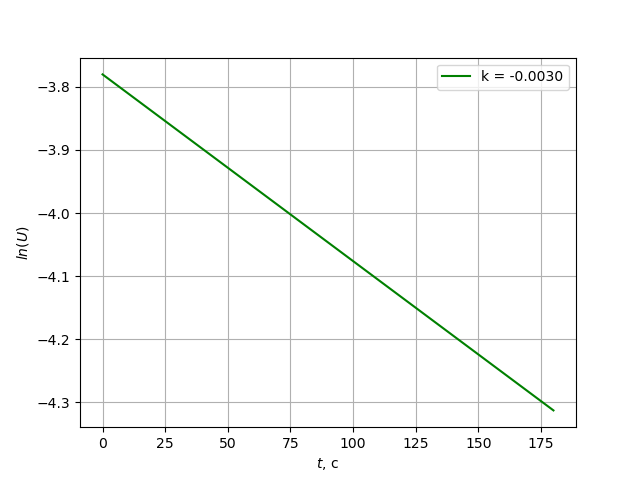
\includegraphics[width=8cm]{plot1.png}
        \subcaption{$\ln (U)(t)$ при $P_1 = 41$ торр}
    \end{subfigure}
    \hfill
    \begin{subfigure}{0.45\textwidth}
        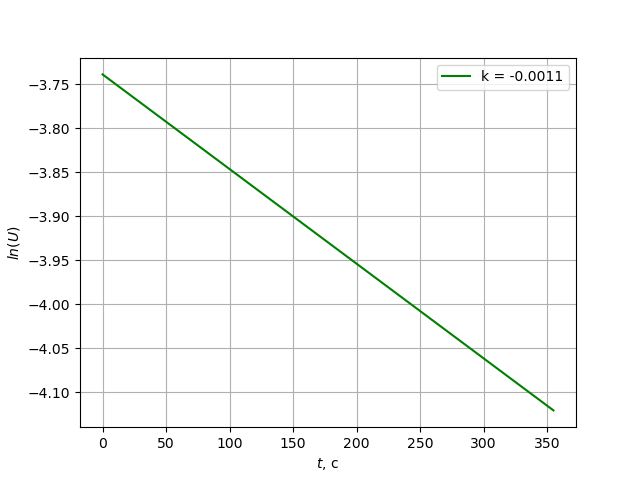
\includegraphics[width=8cm]{plot2.png}
        \subcaption{$\ln (U)(t)$ при $P_2 = 74$ торр}
    \end{subfigure}
    \vfill
    \begin{subfigure}{0.45\textwidth}
        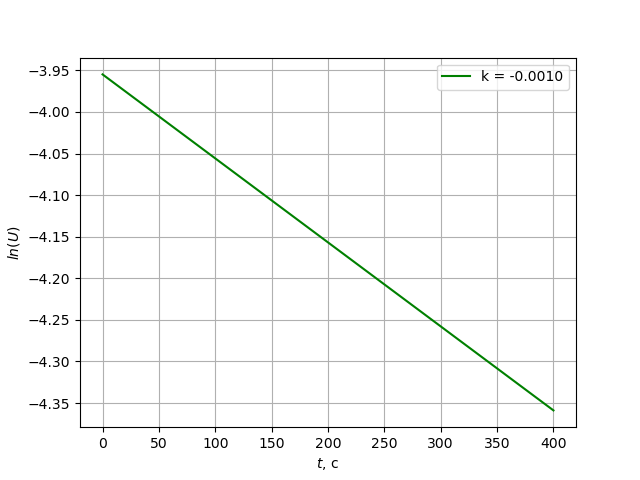
\includegraphics[width=8cm]{plot3.png}
        \subcaption{$\ln (U)(t)$ при $P_3 = 120$ торр}
    \end{subfigure}
    \hfill
    \begin{subfigure}{0.45\textwidth}
        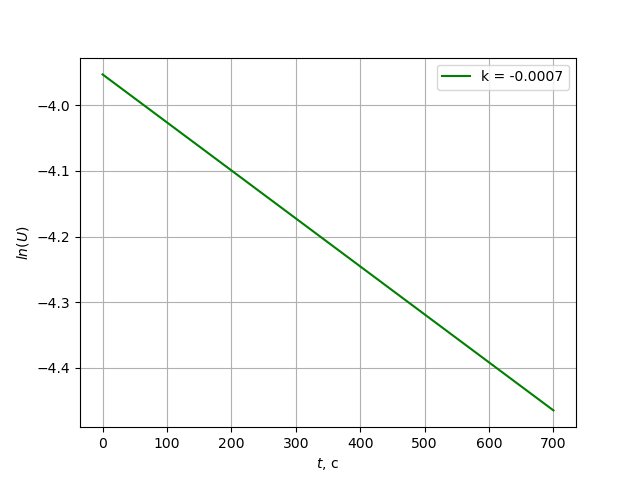
\includegraphics[width=8cm]{plot4.png}
        \subcaption{$\ln (U)(t)$ при $P_4 = 155$ торр}
    \end{subfigure}
\end{figure}


\begin{wrapfigure*}
    \centering
    \begin{minipage}{0.45\textwidth}
        \centering 
        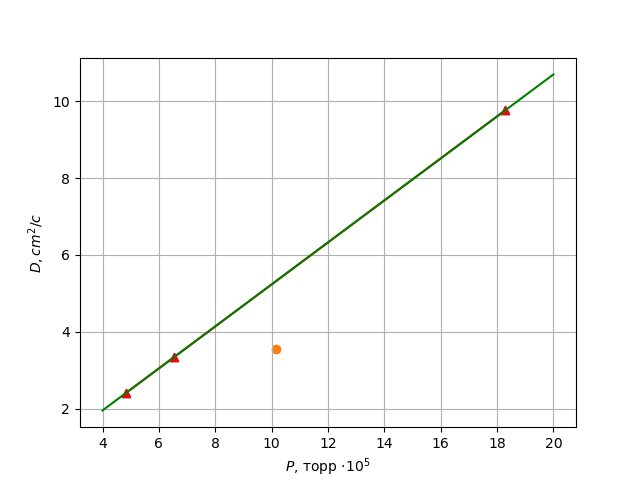
\includegraphics[height=7cm]{DP_plot.png}
        \caption{Зависимость $D(\frac{1}{P})$ коэффициента взаимной диффузии от давления}
    \end{minipage}
\hfill
    \begin{minipage}{0.48\textwidth}
        \centering
        \begin{tabular}{|c|c|c|c|c|}
            \hline
            $P$, торр  & 41 & 74 & 120 & 155\\\hline
            $D$, $\frac{\text{см}^2}{c}$ & 9.77 & 3.55 & 3.33 & 2.41\\\hline
            $\lambda$, мм$\cdot 10^{-3}$ & 2.35 & 0.86 & 0.8 & 0.58\\\hline 
        \end{tabular}
        \caption{Зависимость давления от коэффициента взаимной диффузии}
    \end{minipage}
\end{wrapfigure*}
\newline
Экстраполируя полученную зависимость, находим значение коэффициента 
взаимной диффузии гелия с воздухом при атмосферном давлении и 
комнатной температуре $D = 0.31$ см$^2$/c. Табличное значение этой
величины при $0^{\circ}$C 0.62 см$^2$/с. 

